\label{sec:results}
\providecommand{\nym}{{\color{red}\bfseries [NOT YET MEASURED]}}
\providecommand{\xh}{x_{\mathrm{h}}}
% Placeholder for a measurement that is defined by the protocol but was not carried out.
\providecommand{\NoHumanPanel}{%
\textbf{Not carried out.} The blind human panel of eight raters, the Fleiss kappa
agreement measure and the live demonstration of the proposal were not executed,
so the third and fourth sub-tests of this qualification test remain
\nym{}. The feature-correlation and overlay sub-tests above measure geometric and
pixel-domain distances between the synthesis and the writers' real hands. No
measurement of human acceptance of the output was taken, and the proposal's
demonstration asks for one; Section~\ref{sec:discussion} treats what that
leaves unproven.}

\subsection{Summary of results achieved} % REQUIRED HEADING
\label{sec:res-summary}

This section qualifies the system against requirements R1 to R6 and field conditions FC1 and FC2 of the approved proposal.
All measurements were taken on the development laptop (x86-64, CPython), not on the ODROID N2+, and every figure states its data set and split.
Table~\ref{tab:res-summary} uses four status labels: \emph{Met}, \emph{Partially met}, \emph{Not met} and \emph{Not measured}.
A requirement is met only where the evidence bears directly on it, and a cell states where a figure came from a split that favours the system or from a judge that also takes part in the synthesis search.
Thirteen writers were used, eight from IAM and five personal contributors, three more than R6 requires, but not every measurement covers all thirteen and the difference matters: the qualification-test harness was configured for ten, omitting the three weakest writers for shape-based identification.
Each cell therefore states the writer count that its figure actually covers, and names the model checkpoint it was measured with, because the checkpoint the live server loads is not the one most of the accuracy figures were taken on.
Section~\ref{sec:res-qtp} states both qualifications and Appendix~\ref{sec:app-prov} traces them to the stored files.

\begin{table}[h]
\centering
\fontsize{10}{12}\selectfont
\begin{tabularx}{\linewidth}{|>{\raggedright\arraybackslash}p{4.6cm}|>{\raggedright\arraybackslash}X|>{\raggedright\arraybackslash}p{2.3cm}|}
\hline
\textbf{Intended outcome} & \textbf{Actual outcome} & \textbf{Location in report} \\
\hline
\multicolumn{3}{|l|}{\textbf{Core mission requirements and specifications}} \\
\hline
R1: Reproduce text in the style of any writer of the training set, at least 85\% character accuracy and 85\% stylistic correlation. &
\textbf{Partially met.} Character accuracy of the synthesised text was 82.2\% (thirteen writers, 6 sentences, 2 seeds, $N{=}30$) and 79.2\% at $N{=}8$, both read by the \texttt{paper\_cnn\_bilstm\_ctc\_joint\_best} checkpoint; style correlation over nine geometric features was 0.714, measured on the ten-writer qualification-test subset (Abhinav, Owen and Thiya excluded). Both are below the 0.85 target. The visible-match assessment that the proposal asks for was not carried out. &
Qualification test 1 \\
\hline
R2: Decode the text and identify the writer with an overall accuracy of at least 95\%. &
\textbf{Partially met.} 98.61\% character and 94.21\% word accuracy over 669 real line crops (\texttt{paper\_cnn\_bilstm\_ctc\_joint\_best}, greedy CTC, no beam search and no lexicon); the writer of 1358 real lines was identified at 99.78\% by the ink classifier (\texttt{author\_classifier\_10new\_weights}) and 93.67\% by the shape classifier (\texttt{author\_shape\_10new\_weights}), per line, not per page. The crops were correctly cut and their writers appear in the fine-tuning data, so the split is optimistic, and the complete page-to-text chain was not measured. &
Qualification test 2 \\
\hline
R3: Reproduce text at no more than 4~s per character. &
\textbf{Not met.} A four-character word at $N{=}6$ took 64.3~s to a rendered preview, which is 16.1~s per character against the 4~s limit. The physical drawing time was not measured, because the gantry bring-up was not completed. &
Qualification test 3 \\
\hline
R4: Identify the writer and decode the text within $2+0.025x$~s for $x$ characters. &
\textbf{Partially met.} Recognition ran at 8.86~ms per character against the 25~ms allowance, and the whole page took 40.3 to 100.1~s against a budget of 26.4 to 43.9~s, a factor of 1.15 to 2.98. Segmentation dominates it: 24.8 to 69.1~s per page, timed on \texttt{SegmentPage.ProcessPage}, the \emph{retired} segmenter, not on the deployed \texttt{SegmentLean.py}. Nothing was timed on the ODROID N2+. &
Qualification test 4 \\
\hline
R5: Absolute gantry positional error of at most 0.5~mm. &
\textbf{Not measured.} The commanded position quantises to 12.5~\textmu m per step, far finer than the tolerance, but no drawn mark was measured. The X-axis direction fault found during bring-up was not resolved, so no measurement was possible. &
Qualification test 5 \\
\hline
R6: At least 10 writing styles trained and stored permanently. &
\textbf{Partially met.} Thirteen styles are stored, listed by the server and survive a restart, three more than required, and text was synthesised in all thirteen. Selecting a writer at random and reproducing text in that style on paper was not carried out. &
Qualification test 6 \\
\hline
\multicolumn{3}{|l|}{\textbf{Field condition requirements and specifications}} \\
\hline
FC1: Operation in well-lit areas, 400 to 1000~lux. &
\textbf{Not measured.} No illuminance was recorded at the page plane. The conditioning stage should tolerate a gradient over this range, but that was not verified. &
Section~\ref{sec:res-fc} \\
\hline
FC2: Operation on a stable, level, vibration-free surface. &
\textbf{Not measured.} No tilt or vibration measurement was recorded. &
Section~\ref{sec:res-fc} \\
\hline
\end{tabularx}
\caption{Summary of results achieved.}
\label{tab:res-summary}
\end{table}

R6 is met, and R2 is met for writer identification on real handwriting.
R1 is close but not at its target, the shortfall lying in word-level rather than character-level accuracy; R3 fails on the search cost and R4 on segmentation rather than recognition.
R5 and both field conditions could not be assessed, because the hardware bring-up and the environmental measurements were not completed.
Figure~\ref{fig:res-bars} places each measured value against its target, and Section~\ref{sec:discussion} analyses the shortfalls.

\subsection{Qualification tests} % REQUIRED HEADING
\label{sec:res-qtp}

For each requirement, this subsection summarises the test that is to prove it, in the proposal's order of importance; each test carries its own metric definitions, numbered step list and, where one was prepared, its data sheet.

\emph{Which writers and which checkpoints.}
Two facts about the data behind this chapter change how every figure in it should be read, and both are traced to their stored evidence in Appendix~\ref{sec:app-prov}.
First, the qualification-test harness covers \emph{ten} of the thirteen stored writers, and the three it omits --- Abhinav, Owen and Thiya --- are exactly the three weakest for shape-based writer identification (Owen 67.6\%, Thiya 93.3\%, Abhinav 97.1\%).
The style correlation, the overlay distances and the independent-judge character accuracy are therefore measured on a subset that favours the system and would be expected to be worse over all thirteen; the search-judge accuracy, the per-writer end-to-end run and the 1358-line writer identification do cover all thirteen, and each figure below is labelled with the writer count it actually covers.
Second, the live server does \emph{not} serve the text checkpoint that most accuracy figures were measured on: it loads \texttt{paper\_cnn\_bilstm\_ctc\_scratch\_best.npz}, \textbf{for which no accuracy was measured} --- \nym{}.
The two writer classifiers it serves are numerically equivalent to the measured ones, so the writer figures transfer to the deployed code and the text figures do not.

\emph{How the figures are computed.}
Every measure quoted in this chapter is defined in full in Appendix~\ref{sec:app-met}, which gives the defining equation of each one, names the routine that implements it and states where a different reading would change the number.
Three of those readings must be known before any figure below is read.
Character accuracy is the Levenshtein accuracy of Equation~\ref{eq:res-cacc}, but a set of lines admits three averages that do not agree (Equation~\ref{eq:res-cacc-avg}): qualification test~1 quotes the \emph{mean over writers} and qualification test~2 the \emph{mean over line crops}, and on the 123 held-out real lines those two readings of the same data differ by 4.7 points.
Word accuracy is the longest-common-subsequence word recall of Equation~\ref{eq:res-wacc} and \emph{not} $1-\mathrm{WER}$, so it charges nothing for inserted words; a reader who assumes $1-\mathrm{WER}$ will take every word figure here as stricter than it is.
Writer accuracy is the per-line form of Equation~\ref{eq:res-wacc-writer} throughout, never the per-page form the proposal's wording implies.
Proportions carry a 95\% Wilson interval (Equation~\ref{eq:res-wilson}) and accuracies a page-level bootstrap, because characters of one page are not independent; a requirement is declared met only if the lower bound exceeds the target.
All text figures come from greedy connectionist temporal classification decoding with no beam search, no language model and no lexicon, and all random choices use recorded seeds.

%%%%%%%%%%%%%%%%%%%%%%%%%%%%%%%%%%%%%%%%%%%%%%%%%%%%%%%%%%%%%%%%%%%%%%%%%%%%%%%%%

\medskip
    \QualificationTest{Reproduction fidelity of the synthesised handwriting (R1)}
\label{sec:res-qtp1}

        \QualificationSection{Objectives of the test or experiment}

            The test is to prove at least 85\% character accuracy and 85\% stylistic correlation.
            The existing evidence is circular, because the networks that select the best of $N$ candidates also score the result; the test therefore uses judges outside the search.
            Sub-tests (b) and (c) and the independent-judge reading of sub-test (a) cover the ten-writer harness subset only, so their values are correct for those ten writers and favourable to the system; the 82.2\% and 79.2\% search-judge figures and the per-writer end-to-end run of Figure~\ref{fig:res-e2e} cover all thirteen.

        \QualificationSection{Equipment used}

            The development laptop (x86-64, CPython) with the thirteen stored style profiles, ten of which the sub-tests exercise; a separate evaluation program, \texttt{qtp\_scripts/qtp1c\_judges.py}, which imports neither the synthesiser nor its judges (its import list is \texttt{qtp\_common}, \texttt{qtp\_lines} and \texttt{np\_inference.text\_model} only), so the independence claim holds literally; and the base recognition checkpoint \texttt{paper\_cnn\_bilstm\_ctc\_hf\_best.pt}, which is not used in the search.
            That checkpoint is a \emph{partially} independent judge, not a fully independent one, and the script says so itself: its \texttt{meta.note} records ``hf checkpoint is a PARTIAL-independent judge (same architecture and data lineage)'', the joint production checkpoint having been trained on from the base model, with the same architecture and the same CTC decoder.
            Stating this strengthens rather than weakens the comparison: it removes the winner's curse of scoring with the very checkpoint that selected the candidate, but not the biases the two networks share, so the 3.7-point drop it measures is a lower bound on the true selection effect.
            The production judge inside the search is \texttt{paper\_cnn\_bilstm\_ctc\_joint\_best.pt}.
            The ODROID N2+ and the gantry were \emph{not} used: everything was produced and scored on the laptop, and no text was written on paper.
            Printed worksheets were prepared for a blind human panel, but the panel was not convened.

        \QualificationSection{Test setup and experimental parameters}

            The sub-tests were run separately.
            Sub-test (a) gives character accuracy twice: by the recogniser inside the search, over thirteen writers, 6 novel sentences and 2 seeds at $N=30$ and over the same writers at $N=8$ in a wider coverage run; and by the base recognition checkpoint \texttt{paper\_cnn\_bilstm\_ctc\_hf\_best.pt}, outside the search, over 60 synthesised lines from the ten-writer subset at $N=20$. Genuine handwriting gives the upper bound, and it comes from two different sets that must not be mixed: the 70-line matched-reference set of \texttt{rewrite\_full.log} (89.0\% character, 70.5\% word) and the 123 held-out lines of \texttt{qtp1c\_results.json} (89.5\% character, 71.3\% word, ten-writer subset). The blind panel of 8 raters and Fleiss' kappa~\cite{fleiss1971} belonged to this sub-test and were not carried out.
            Sub-test (b): nine hand-crafted style features from one deterministic extractor, computed on held-out real pages and on renderings for ten writers; the Pearson correlation $\rho$ of the pooled $z$-scored vectors and a nearest-centroid writer retrieval are reported, bootstrapped over writers.
            Sub-test (c): the sentence a writer actually wrote is synthesised in that writer's style at $N=20$, both images are normalised to a common x-height $\xh$, and the chamfer distance~\cite{barrow1977} and the modified Hausdorff distance~\cite{dubuisson1994} over 30 matched and 300 mismatched pairs are compared by rank-1 retrieval and by the area under the receiver operating characteristic curve (AUC; 0.5 means no writer information)~\cite[p.~868]{fawcett2006}.
            Sub-test (d): the demonstration of the proposal, with 85\% of the produced characters visibly matching. This sub-test was not carried out.

            The metrics of the four sub-tests are the Fleiss kappa of Equation~\ref{eq:res-kappa} for the panel, the Pearson correlation of $z$-scored feature vectors of Equation~\ref{eq:res-pearson} for the style comparison, and the chamfer and modified Hausdorff distances of Equations~\ref{eq:res-chamfer} and~\ref{eq:res-mhd} with the AUC of Equation~\ref{eq:res-auc} for the overlay; all four are defined in Appendix~\ref{sec:app-met}, together with the normalisation that the overlay applies to both images before they are compared (Figure~\ref{fig:res-overlay}).
            Two deviations from the protocol matter to the figures below.
            The correlation actually measured used the nine geometric features of Table~\ref{tab:res-r1} rather than the seven that the protocol prescribes (Table~\ref{tab:res-features}), and the overlay was run over ten writers and three sentences each, giving the 30 matched and 300 mismatched pairs reported here instead of the 40 and 360 the protocol sized it at.
            Table~\ref{tab:res-panel} is the worksheet each of the 8 raters was to complete, which carries no indication of whether a line is synthesised or genuine; the worksheets were printed but all remained blank.

        \QualificationSection{Steps followed in the test or experiment}

            The protocol has seven steps: (1) fix the held-out pages and freeze the system; (2) produce the 150 renderings (direct and G-code replay) and store writer, sentence, seed and text; (3) read every rendering with the base recogniser and evaluate Equation~\ref{eq:res-cacc} with the intervals; (4) run the panel with the worksheet of Table~\ref{tab:res-panel}, computing transcription accuracy and the kappa of Equation~\ref{eq:res-kappa}; (5) run the feature extractor of Table~\ref{tab:res-features} and compute the correlation of Equation~\ref{eq:res-pearson} together with the confusion matrix; (6) compute the overlay distances of Equations~\ref{eq:res-chamfer} and~\ref{eq:res-mhd} by the procedure of Figure~\ref{fig:res-overlay}, the AUC of Equation~\ref{eq:res-auc} and the rank-1 retrieval, and produce overlay figures for at least four sentences; (7) write a sentence on the gantry in a chosen style and count visibly matching characters (pass at 85\%).
            Steps (1) to (3), (5) and (6) were carried out, on the development laptop and not on the ODROID N2+ that the protocol names; the confusion matrix, overlay figures and intervals come from stored outputs.
            Steps (4) and (7) were \emph{not} carried out, so sub-tests (a) to (c) were evaluated but sub-test (d) was not.
            The protocol for step (4) was that the raters be 8 persons who are neither the student nor writers in the data set, the panel blind and working from 30 synthesised lines (3 per writer) and 10 genuine control lines in random order, about 1350 scored characters per rater; none of this took place.

        \QualificationSection{Results or measurements}

            Table~\ref{tab:res-r1} lists the measured figures in two groups: those from the \emph{search judges}, the recogniser and writer classifier that score the $N$ candidates, which the selection inflates; and the \emph{independent measurements}, namely the style correlation on geometric features, the overlay test in the pixel domain and a character-accuracy reading by a checkpoint that was \emph{not} used in the search, none of which involves the search and all of which can therefore fail.
            Figure~\ref{fig:res-overlay-examples} is the worked overlay of one sentence, which is the sub-test the eye can check directly.
            The breakdowns behind the summary rows are in Appendix~\ref{sec:app-res}: the per-feature correlation (Figure~\ref{fig:res-features} and Table~\ref{tab:res-perfeature}), the character accuracy under both checkpoints (Figure~\ref{fig:res-judges}), the overlay distance distributions (Figure~\ref{fig:res-dist}), genuine handwriting against the synthesis of the same sentences (Figure~\ref{fig:res-matched}) and the end-to-end result per writer (Figure~\ref{fig:res-e2e}).

\begin{table}[h]
\centering
\fontsize{9.5}{11.5}\selectfont
\begin{tabularx}{\linewidth}{|>{\raggedright\arraybackslash}p{4.6cm}|>{\raggedright\arraybackslash}X|>{\raggedright\arraybackslash}p{2.0cm}|}
\hline
\textbf{Measure} & \textbf{Measured value, data set and caveat} & \textbf{Circular?} \\
\hline
Character accuracy, search judges & 82.2\% over 13 writers, 6 novel sentences $\times$ 2 seeds, best-of-30; 79.2\% at best-of-8. Read by \texttt{paper\_cnn\_bilstm\_ctc\_joint\_best}, the checkpoint inside the search. & Yes \\
\hline
Character accuracy, \emph{partially independent} judge & 81.2\% (mean over writers) over 60 synthesised lines (the ten-writer subset, 6 sentences, best-of-20), read by \texttt{paper\_cnn\_bilstm\_ctc\_hf\_best}, a checkpoint not used in the search but of the same architecture and data lineage. Word accuracy 42.0\% by Equation~\ref{eq:res-wacc}. & No \\
\hline
Character accuracy, \emph{real} handwriting of the same words & Two distinct runs, not to be mixed. (i) The matched-reference set: 89.0\% character and \textbf{70.5\%} word over \textbf{70} lines (\texttt{rewrite\_full.log}, thirteen writers). (ii) The held-out line set: \textbf{89.5\%} character and 71.3\% word over \textbf{123} lines (\texttt{qtp1c\_results.json}, joint checkpoint, ten-writer subset, charset-filtered). Earlier drafts paired the 89.0\% of (i) with the 71.2\% line-mean word accuracy of (ii), which is the source of the 70.5-against-71.2 word-accuracy discrepancy noted elsewhere in this report: the two numbers are two different sets, not two readings of one. The upper bound the synthesis is trying to reach is 89.0 to 89.5\% character either way. & No \\
\hline
Writer identification on synthesised text & 80.1\% (official run), 89.7\% through G-code in the coverage run, by the shape classifier. & Yes \\
\hline
Writer identification on real handwriting (same classifier) & 93.7\% over 1358 real lines (ink classifier 99.8\%). & No \\
\hline
\textbf{Style correlation} $\rho$ on nine geometric features & \textbf{0.714} for shape-only features (95\% bootstrap 0.612 to 0.859 over writers) and 0.701 for all features, on the held-out page set; 0.776 and 0.697 on the all-pages set. \textbf{Below the 0.85 target.} & No \\
\hline
Style correlation, per feature (Pearson $r$ across writers) & Best slant 0.996 and ascender extent 0.974; worst descender extent 0.148 and ascender-to-descender ratio 0.509. All nine coefficients are in Table~\ref{tab:res-perfeature}. & No \\
\hline
Overlay test, matched against mismatched pairs (30 lines, best-of-20) & Chamfer distance ratio 0.454, modified Hausdorff 0.369; rank-1 writer retrieval 20.0\% and 23.3\% against a chance of 10\%; AUC 0.707 and 0.722. & No \\
\hline
Word accuracy, search judges & 48.9\% (official run), 44\% (coverage run); 41.6\% with the partially independent judge; 70.5\% for real handwriting of the same words over the 70-line matched-reference set and 71.3\% over the 123 held-out lines. All are the longest-common-subsequence word recall of Equation~\ref{eq:res-wacc}, not $1-\mathrm{WER}$. & Mixed \\
\hline
\end{tabularx}
\caption{Results for qualification test 1 (measured on the development laptop). The writer count differs by row and is stated in each: the search-judge and real-handwriting rows cover all thirteen writers, whereas the style-correlation, overlay and independent-judge rows cover only the ten-writer harness subset, which omits the three weakest writers on the shape judge. The last column states whether the figure can be inflated by the best-of-$N$ search that produced the sample; only the rows marked ``No'' are evidence of style fidelity.}
\label{tab:res-r1}
\end{table}




\begin{figure}[h]
\centering
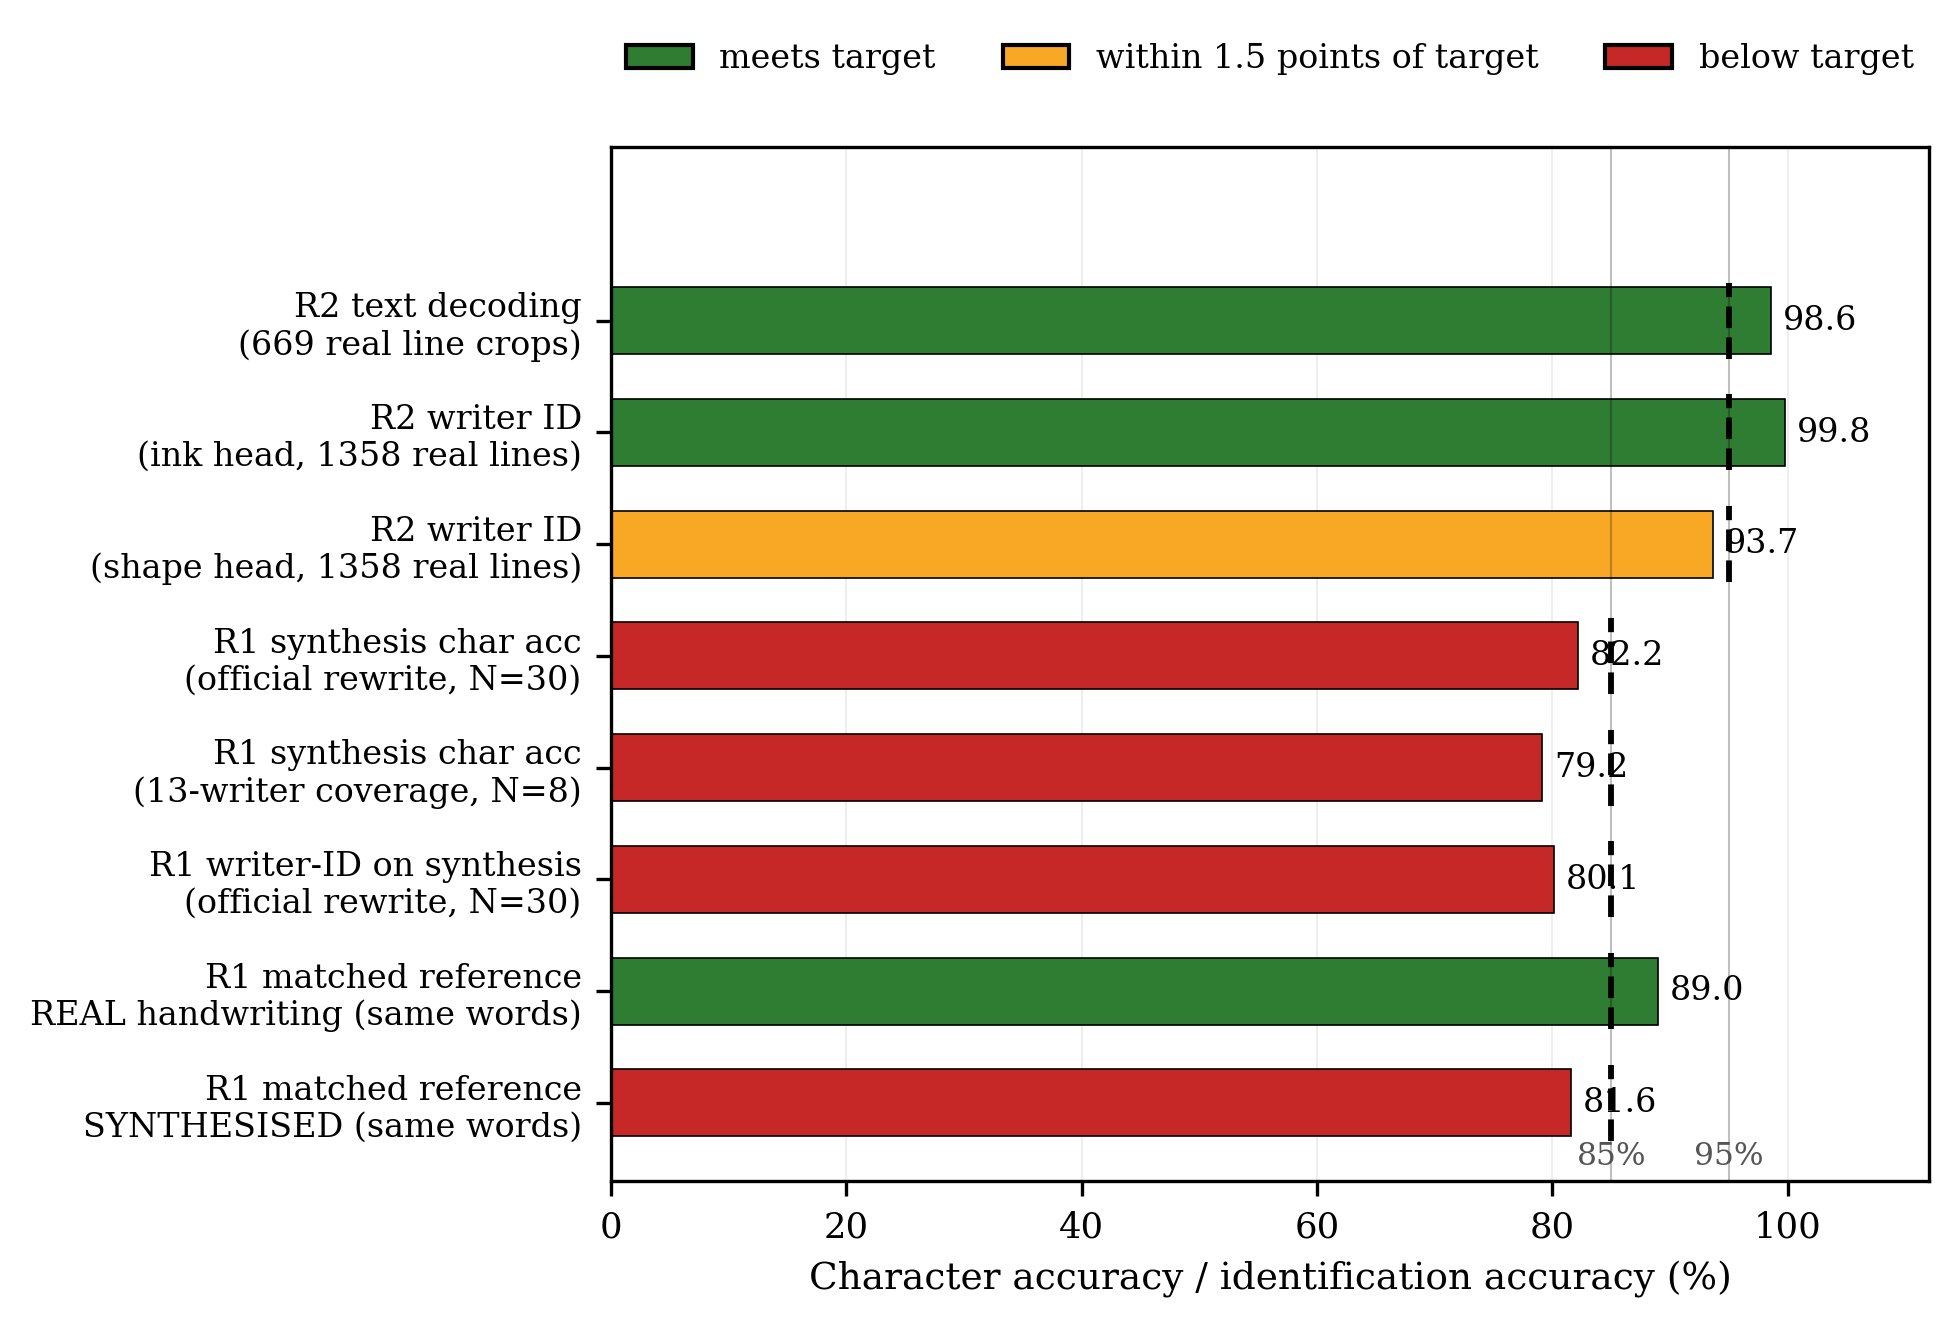
\includegraphics[width=0.85\linewidth]{Figures/res_requirements_vs_achieved.png}
\caption{Measured accuracy against the target of each requirement. Targets are marked by the dashed vertical lines at 85\% (R1) and 95\% (R2). Green bars meet the target, amber bars lie within 1.5 points of it, and red bars fall below it. The two green R1 bars are the matching comparison on genuine handwriting and the writer classifier on real lines; the red synthesis bars are the values the system actually produces.}
\label{fig:res-bars}
\end{figure}

\begin{figure}[h]
\centering
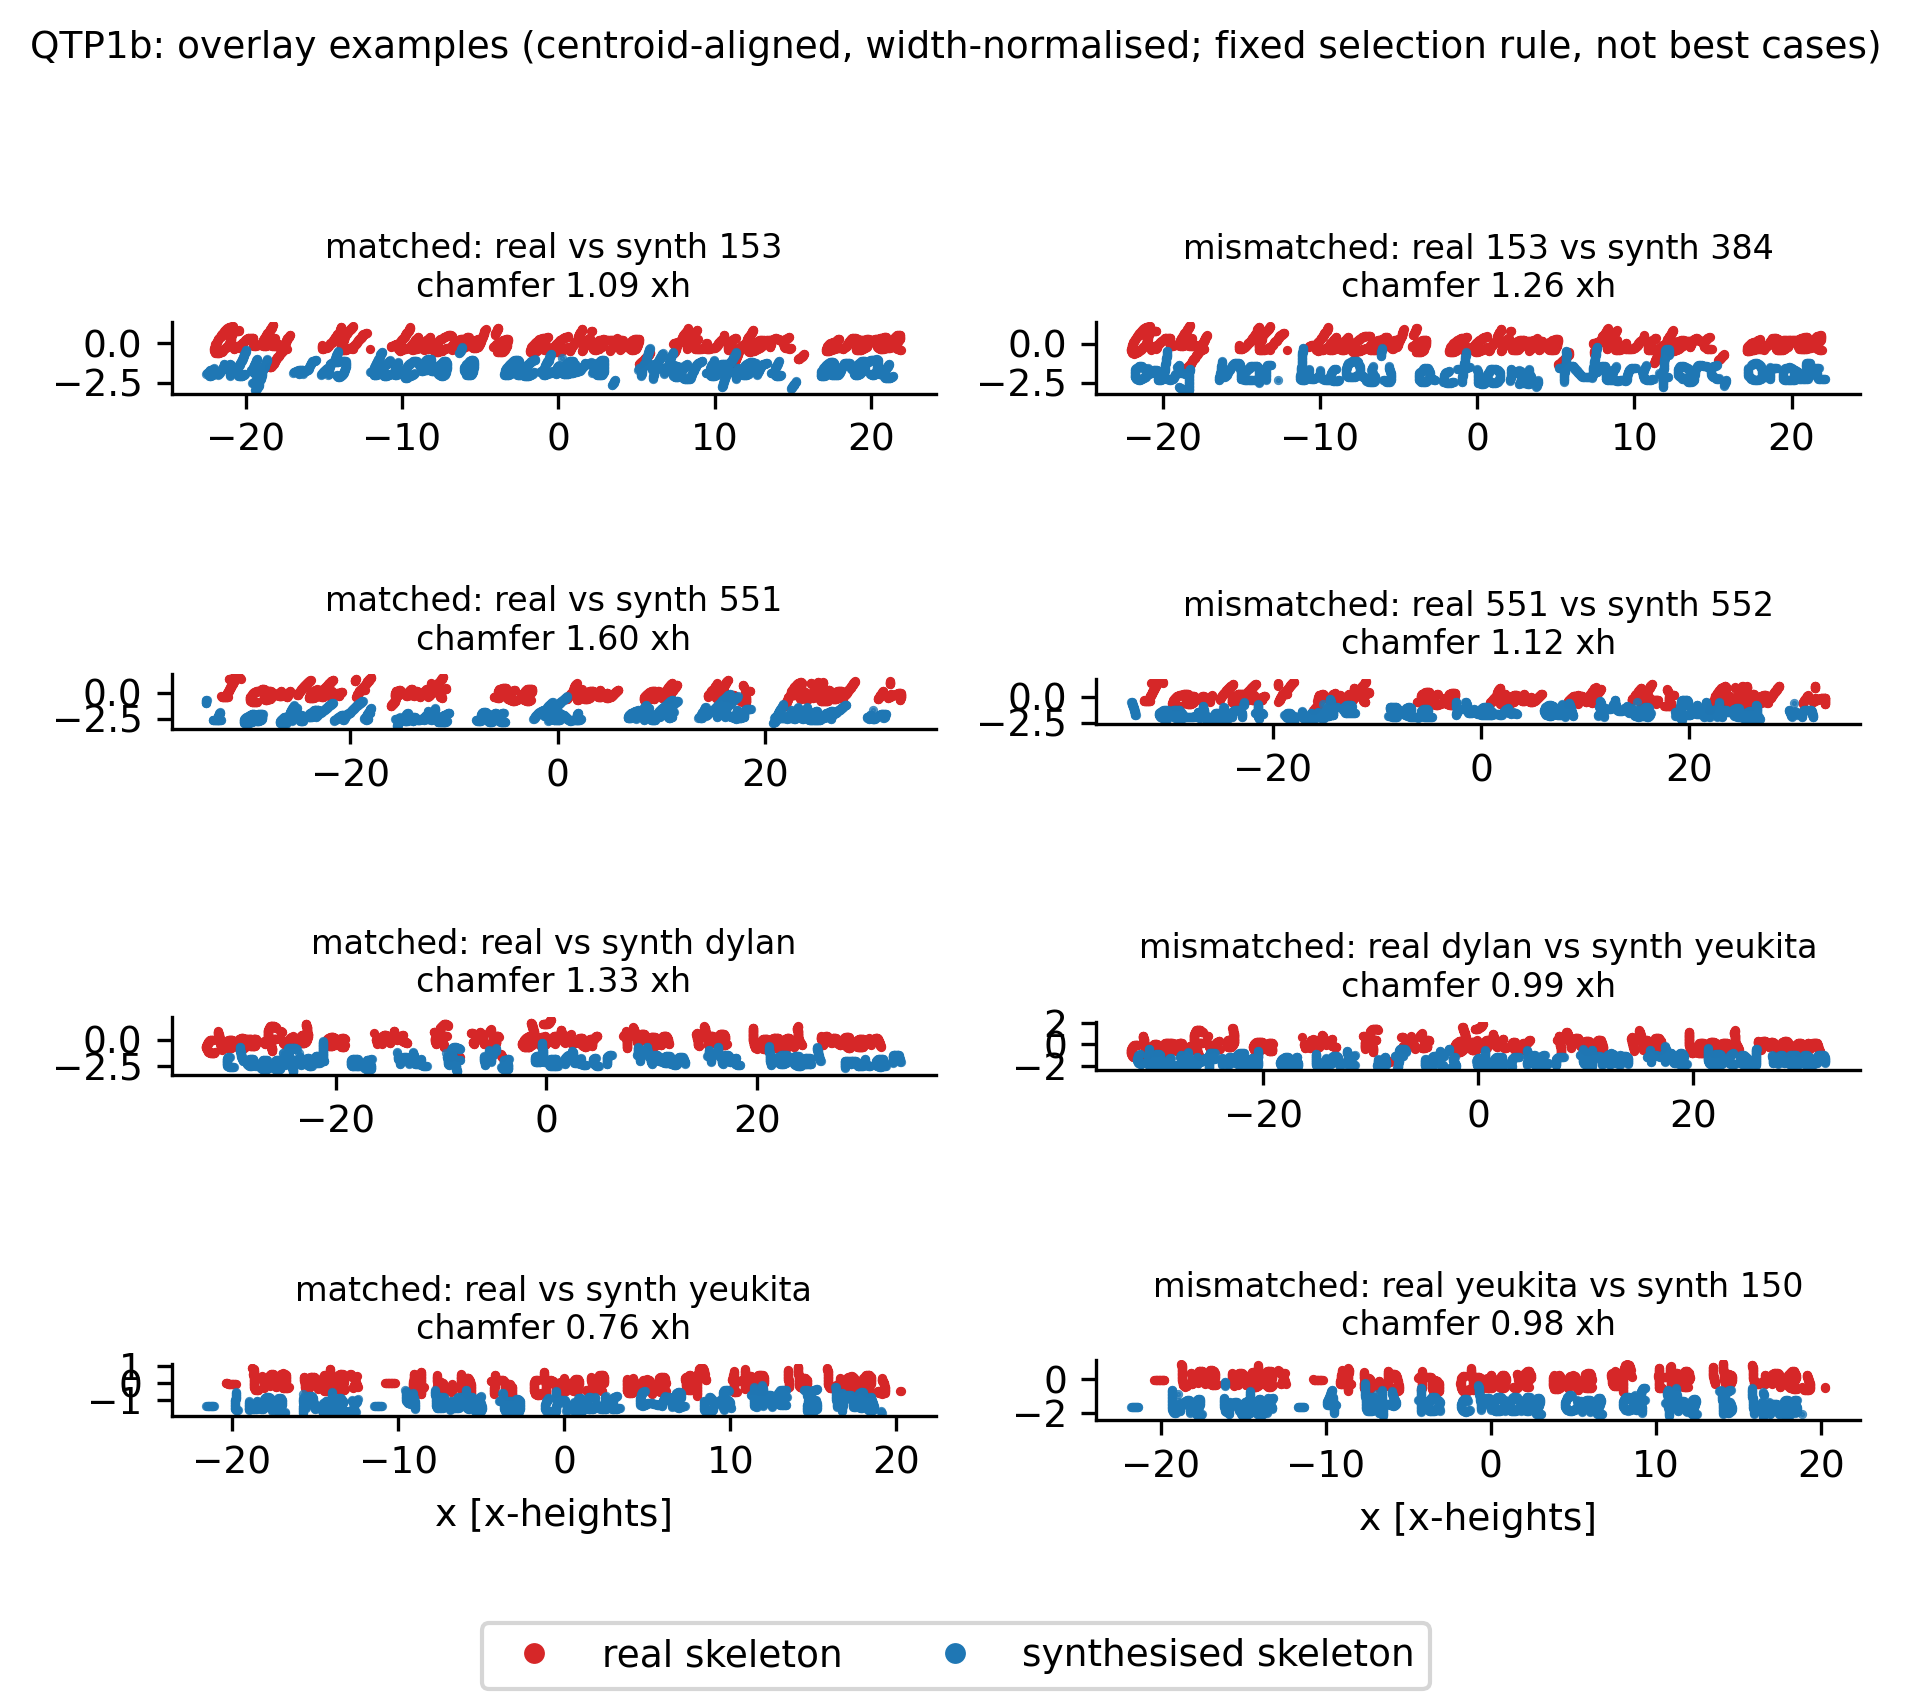
\includegraphics[width=0.85\linewidth]{Figures/qtp1_overlay_examples.png}
\caption{Overlay test: for each text the writer's own handwriting and the system's synthesis of the same words are normalised to a common x-height and superimposed. Matched pairs are visibly closer than mismatched pairs, which is what the distance ratios and the rank-1 retrieval rate of 20\% (chance 10\%) measure. The procedure that produces these overlays is given as Figure~\ref{fig:res-overlay}.}
\label{fig:res-overlay-examples}
\end{figure}


        \QualificationSection{Observations}

            The nine-feature style correlation was 0.714 on shape-only features, below the 0.85 target, with a bootstrap interval over writers of 0.612 to 0.859.
            Per feature it was highest for slant (0.996) and ascender extent (0.974) and lowest for descender extent (0.148), the ascender-to-descender ratio (0.509) and the word gap (0.605), that is for the extents below the baseline and for the spacing. The word-accuracy gap between the synthesis and real handwriting of the same words was 23.8 points.
            The overlay test gave an AUC of 0.71 against 0.5 for no writer information, and rank-1 retrieval of 20\% against a chance of 10\%.
            A partially independent checkpoint read the synthesised lines 3.7 points below the production checkpoint, 81.2\% against 84.9\% as a mean over writers, on the same 60 lines at best-of-20 (\texttt{meta.nTries\_in\_synthesis} is 20 in \texttt{qtp1c\_results.json}); the two-judge pair is therefore (84.9, 81.2) at $N=20$, and not a best-of-30 comparison.
            Against the real-ink ceiling, the production checkpoint read genuine handwriting of the same words at 89.0\% over the 70-line matched-reference set and 89.5\% over the 123 held-out lines, about 8 points above the independent judge's reading of the synthesis.
            Part of that gap is the judge and not the synthesis: on the same 123 real lines the independent checkpoint itself reads only 86.6\% against the production checkpoint's 90.2\% (both means over writers), so its own penalty on real ink is about 3.6 points.
            All of these readings cover the ten-writer subset.
            An earlier comparison measured 75.9\% before the search was introduced and 81.6\% after it.
            \NoHumanPanel


        \QualificationSection{Statistical analysis}

            By the Wilson interval of Equation~\ref{eq:res-wilson}, the official run's 82.2\% over 156 sentences has a lower bound near 75\%, so the result is below 85\% and not a sampling fluctuation.
            The style correlation is bootstrapped over writers (2000 resamples), the correct unit because the nine features are measured per writer, and the overlay AUC over 30 matched and 300 mismatched pairs.
            The two-judge comparison is paired, both checkpoints reading the same 60 synthesised lines, so the 3.7-point difference is not affected by sampling variation in the output.
            The proportion of characters a human observer would accept as matching the writer's style, which is how the proposal worded the demonstration, was not measured.

%%%%%%%%%%%%%%%%%%%%%%%%%%%%%%%%%%%%%%%%%%%%%%%%%%%%%%%%%%%%%%%%%%%%%%%%%%%%%%%%%

\medskip
    \QualificationTest{Classification of text and writer from real photographed pages (R2)}
\label{sec:res-qtp2}

        \QualificationSection{Objectives of the test or experiment}

            The test is to prove an overall accuracy of at least 95\% through the whole chain on pages never used for training, checkpoint selection or tuning.
            As the proposal does not define ``overall'', text accuracy $A_{\mathrm{c}}$ (Equation~\ref{eq:res-cacc}) and writer accuracy $A_{\mathrm{w}}$ (fraction of pages assigned to the correct writer) are reported separately and combined as
            \begin{equation}
            \label{eq:res-overall}
            A_{\mathrm{mean}}=\tfrac{1}{2}\left(A_{\mathrm{c}}+A_{\mathrm{w}}\right),\qquad A_{\mathrm{prod}}=A_{\mathrm{c}}\,A_{\mathrm{w}},
            \end{equation}
            where $A_{\mathrm{prod}}$ (both correct) is the criterion and $A_{\mathrm{mean}}$ the lenient reading.

        \QualificationSection{Equipment used}

            The capture rig and its camera photographed the pages of the five personal writers. Segmentation, recognition and writer classification then ran on the development laptop with the final server and models; the ODROID N2+ produced no figure in this test. Camera and lamp: \mustdo{camera model, resolution, mounting height, lamp type and photograph of the rig}.

        \QualificationSection{Test setup and experimental parameters}

            The line-level validation split of the personal writers leaks: a random 15\% of lines per page was held out, so lines from the same sheet and session are in both sets (52 of 123 validation lines share pages with training), and the checkpoint was selected on them.
            The fix is new pages kept aside: at least 3 per personal writer, plus the held-out form page of each of the eight database writers, photographed with the rig (about 14 pages, 350 lines). Seen lines are scored separately to quantify the leakage, and references are double-entered transcripts.

        \QualificationSection{Steps followed in the test or experiment}

            Each frozen photograph is classified through the server without intervention; line text, per-line probabilities and page-level mean probabilities are recorded, scored and summarised in a $10\times10$ confusion matrix, and the predefined paragraph is then classified live.

        \QualificationSection{Results or measurements}

            Table~\ref{tab:res-r2} lists the measured figures. Text and writer accuracy are separate, with Equation~\ref{eq:res-overall} combining them where both exist.

\begin{table}[h]
\centering
\fontsize{10}{12}\selectfont
\begin{tabularx}{\linewidth}{|>{\raggedright\arraybackslash}p{4.9cm}|>{\raggedright\arraybackslash}X|}
\hline
\textbf{Measure} & \textbf{Measured value, data set and caveat} \\
\hline
Recogniser, character accuracy & 98.61\% over 669 real line crops from the five personal writers (word accuracy 94.21\%). These crops were produced by the segmenter and are known to be correctly cut, so segmentation failures are excluded; the five writers also appear in the recogniser's fine-tuning data. \\
\hline
Recogniser, per writer & Owen is the strongest at 99.15\% and Thiya the weakest at 96.46\% character accuracy, over 75 to 206 crops each; the full breakdown is Table~\ref{tab:res-perwriter}. \\
\hline
Writer identification, ink classifier & 99.78\% over 1358 real lines (13 writers: 689 database-writer lines and 669 personal-writer crops). Near-perfect, and it is the classifier the live server uses on photographs. \\
\hline
Writer identification, shape classifier & 93.67\% over the same 1358 lines, against 83.36\% before a training fault was corrected (Section~\ref{sec:res-qtp1}). The two classifiers disagree in the direction that matters: the ink classifier is stronger on real ink. \\
\hline
Per-writer detail & Figure~\ref{fig:res-writerid}. Eight writers are at 98.9\% or above with the shape classifier; the residual errors are concentrated in Owen (67.6\%), Dylan (84.7\%) and Thiya (93.3\%). \\
\hline
Live server classification, one crop & \textbf{One} detected line, the correct writer (Owen) at \textbf{89.4\%} confidence, with the next candidate (Dylan) at 10.5\%, and a near-correct transcription (``Vloggers using fame to supfort charities is a positiwe way''). The input was a single already-segmented crop, not a whole photograph, and the call took 2.74~s end to end (\texttt{stage6\_results.json}). A single crop, reported as an illustration and not as a statistic. No whole-page run of the live classify endpoint was recorded: \mustdo{classify a full photographed page through the live server and record \texttt{lines\_detected}, the writer confidence and the transcription, so that a page-level live figure exists.} \\
\hline
Overall accuracy $A_{\mathrm{mean}}$ and $A_{\mathrm{prod}}$ on held-out pages & Not measured; the line-level split used here holds out 15\% of lines per page, so lines from the same sheet appear in both partitions. \\
\hline
\end{tabularx}
\caption{Results for qualification test 2 (13 writers; measured on the development laptop).}
\label{tab:res-r2}
\end{table}


        \QualificationSection{Observations}

            Text decoding reached 98.61\% character accuracy and 94.21\% word accuracy on correctly segmented crops, against the 95\% target, on writers represented in the recogniser's fine-tuning data; writer identification reached 99.78\% with the ink classifier over 1358 real lines from thirteen writers.
            Thiya is the weakest writer for recognition at 96.46\% character accuracy, and Owen, Dylan and Thiya the weakest for shape-based identification.
            Together the two give $A_{\mathrm{mean}}=98.6\%$ and $A_{\mathrm{prod}}=98.4\%$, both above 95\%, on a split that holds out 15\% of lines per page, so lines from the same sheet appear in both partitions.
            Both accuracies are per line and were read by the \texttt{paper\_cnn\_bilstm\_ctc\_joint\_best} text checkpoint and the \texttt{author\_classifier\_10new\_weights} ink checkpoint; the live server serves a different text checkpoint, as Section~\ref{sec:res-qtp} states.
            The one live-server run recorded was a single already-segmented crop: one detected line, the correct writer at 89.4\% confidence, 2.74~s end to end. The 98.6\% figure that belongs to this test is the character accuracy of 669 crops, not a writer confidence.

        \QualificationSection{Statistical analysis}

            With 669 line crops, 98.61\% character accuracy has a Wilson lower bound of about 97.6\%, so the text figure is above 95\% on this data set; 1358 lines at 99.78\% give a lower bound above 99\% for writer identification.
            The stronger caveat is dependence rather than sampling error: lines from one page share a writer, a pen and an illumination, so the effective sample size is nearer the page count than the line count, and the per-page interval would be much wider.
            \emph{Expected outcome on genuinely unseen pages.}
            Both rates are expected to fall, because the ink classifier is sensitive to pen, paper and illumination and the split shares pages between partitions. A defensible figure needs a page-level split with at least three held-out pages per writer, photographed through the rig.

%%%%%%%%%%%%%%%%%%%%%%%%%%%%%%%%%%%%%%%%%%%%%%%%%%%%%%%%%%%%%%%%%%%%%%%%%%%%%%%%%

\medskip
    \QualificationTest{Reproduction time per character (R3)}
\label{sec:res-qtp3}

        \QualificationSection{Objectives of the test or experiment}

            The test is to prove that a sentence of $x$ characters is reproduced within $4x$ seconds,
            \begin{equation}
            \label{eq:res-r3}
            t_{\mathrm{char}}=\frac{T_{\mathrm{syn}}+T_{\mathrm{write}}}{x}\le 4\ \mathrm{s},
            \end{equation}
            where $T_{\mathrm{syn}}$ is the synthesis time and $T_{\mathrm{write}}$ the time from first to last motion.
            As the proposal does not say whether synthesis counts, both variants are reported; calibration is a one-off step, reported separately.

        \QualificationSection{Equipment used}

            The development laptop with the server, and logged time stamps around synthesis. The gantry and a stopwatch were to have given the writing time, but the gantry was not driven, because its bring-up was not completed, so the motion time is a model and not a measurement.

        \QualificationSection{Test setup and experimental parameters}

            The run actually made, recorded in \texttt{qtp\_data/qtp3\_results.json}, used tries $N\in\{1,3,14,30\}$ and five sentences of 22, 40, 58, 83 and 119 characters, with 3, 3, 3 and 2 repetitions for the four values of $N$ respectively (20 cells, 56 syntheses), writer 153 throughout, plus a writer-dependence extra at 58 characters and $N=14$; the writing time is the generator's model for every cell, not a stopwatch reading.
            The protocol as originally written had prescribed $N\in\{1,3,6,14,30\}$, sentences of 10, 20, 40 and 80 characters and 5 repetitions (100 syntheses), with the writing time measured for the 20 jobs at $N=14$; that plan was not the one executed, and the results below are reported against the run that was.
            Only figures measured on the ODROID N2+ itself count; laptop figures are indicative.

        \QualificationSection{Steps followed in the test or experiment}

            After one calibration, each job is synthesised, sent and timed by log and stopwatch, $t_{\mathrm{char}}$ is computed from Equation~\ref{eq:res-r3}, and any stall is kept as a failed run.

        \QualificationSection{Results or measurements}

            Table~\ref{tab:res-r3} and Figure~\ref{fig:res-r3} give the measured figures: a synthesis term that grows with the number of candidates and a writing term that does not.

\begin{table}[h]
\centering
\fontsize{9.5}{11.5}\selectfont
\begin{tabularx}{\linewidth}{|>{\raggedright\arraybackslash}p{4.6cm}|>{\raggedright\arraybackslash}X|}
\hline
\textbf{Measure} & \textbf{Measured value, data set and caveat} \\
\hline
Synthesis time per character, best-of-1 to best-of-30 & Repeated over sentences of 22 to 119 characters and 2 to 3 repetitions per cell, on the development laptop. At best-of-1 the synthesis costs about 0.4 to 0.7~s per character; at best-of-14 about 0.9 to 1.8~s per character; at best-of-30 about 1.8 to 3.4~s per character. \\
\hline
G-code generation & 0.006 to 0.014~s per sentence, i.e.\ negligible at any sentence length. \\
\hline
Preview rendering and read-back & About 0.02 to 0.05~s and 0.6 to 0.8~s per sentence respectively; both are small beside the synthesis term. \\
\hline
Physical writing time, from the generator's own model & 88.7~s for a 22-character sentence and 154.4~s for a 58-character sentence, i.e.\ about 2.7 to 4.0~s per character, against the 4~s limit \emph{for the writing alone}. \\
\hline
Total per character at best-of-14 & Figure~\ref{fig:res-r3}: synthesis contributes about 1.0 to 1.8~s and writing about 2.7 to 4.0~s, so the total lies between about 4 and 6~s per character and straddles the limit. \\
\hline
Live server measurement, four-character word, best-of-6 & 64.3~s from request to rendered preview, i.e.\ 16.1~s per character. A very short sentence is the worst case because the per-job costs (model loading, segmentation of the uploaded image) are amortised over only four characters. \\
\hline
Physical writing time measured on the gantry & Not measured; the gantry bring-up was not completed, so no drawn job was timed. The figures above are the generator's model, not observations. \\
\hline
Timing on the ODROID N2+ & Not measured. \\
\hline
\end{tabularx}
\caption{Results for qualification test 3 (development laptop; the writing figures are model values, not measurements).}
\label{tab:res-r3}
\end{table}

\begin{figure}[h]
\centering
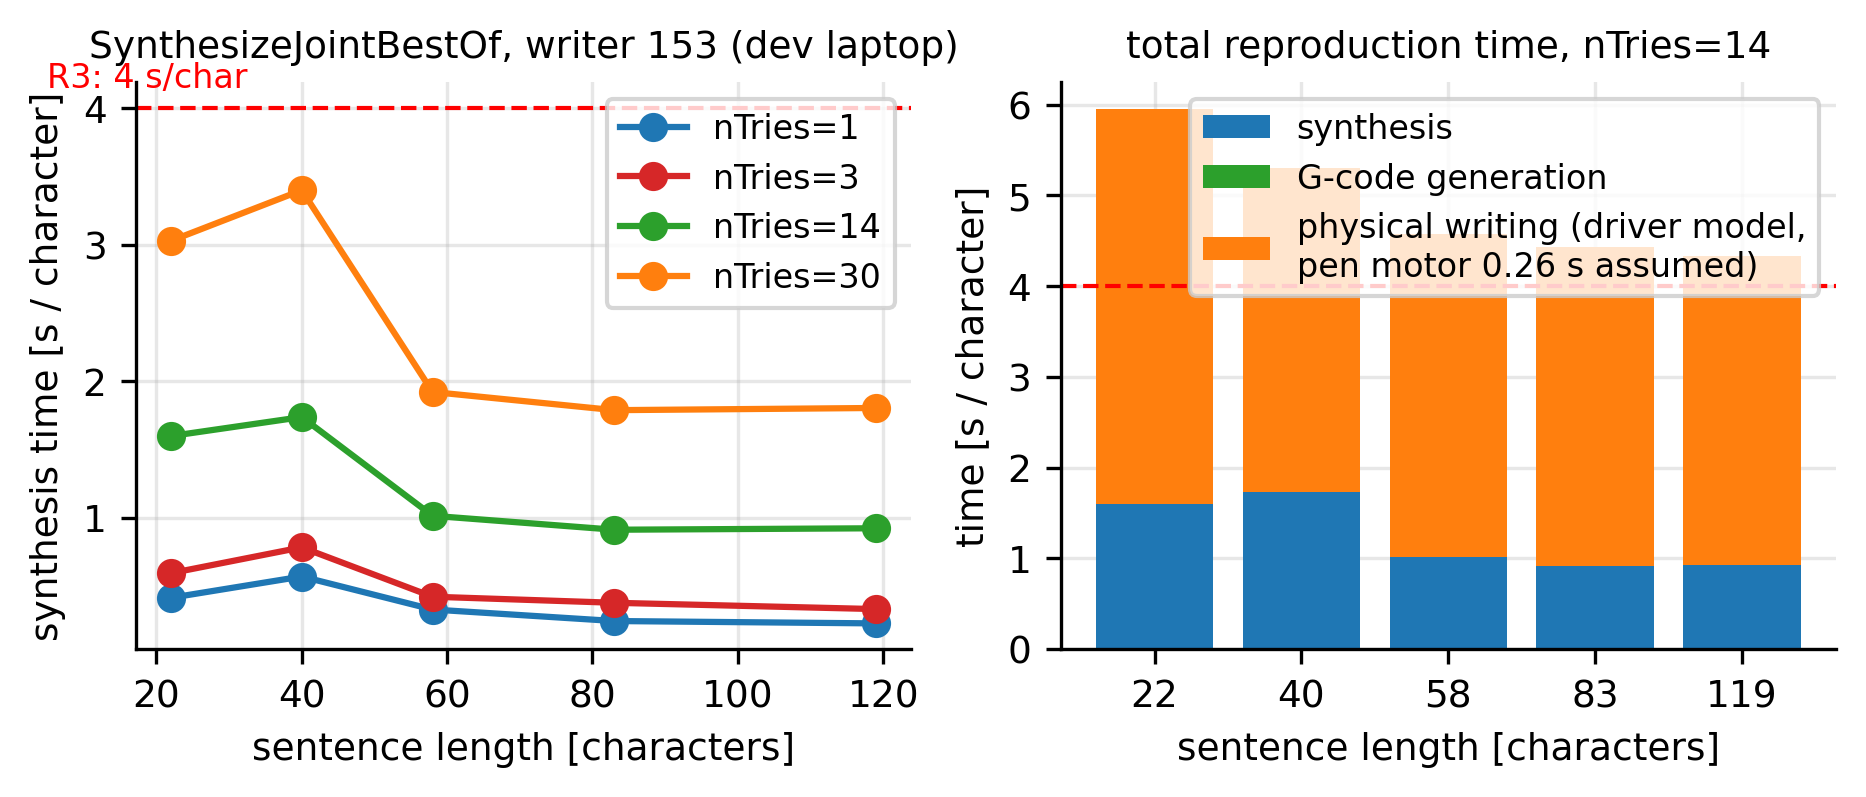
\includegraphics[width=0.85\linewidth]{Figures/qtp3_timing_breakdown.png}
\caption{Reproduction time against the 4~s per character limit of R3. Left: synthesis time per character against sentence length for four values of the number of candidates. At best-of-1 and best-of-3 the synthesis alone is comfortably inside the limit; at best-of-30 it approaches and crosses it. Right: total time per character at best-of-14, decomposed into synthesis, G-code generation and the physical writing time predicted by the generator's model. The writing term, not the synthesis term, is the larger contributor and is what pushes the total past the limit.}
\label{fig:res-r3}
\end{figure}

        \QualificationSection{Observations}

            The synthesis cost stayed well under 1~s per character up to best-of-3 and grew in proportion to the number of candidates, from about 0.4 to 0.7~s per character at best-of-1 to about 1.8 to 3.4~s at best-of-30.
            The generator's model gives 2.7 to 4.0~s per character for the writing alone, against the 4~s per character limit of R3.
            The four-character word at best-of-6 gave 16.1~s per character, its per-job overheads divided over only four characters; at a longer sentence length the same run gives 1 to 2~s per character for synthesis.
            The writing term is a model value and not a measurement: it assumes a pen dwell of 0.26~s per stroke, and no drawn job was timed on the gantry.

        \QualificationSection{Statistical analysis}

            Each cell is the mean of two or three repetitions, and the table quotes a range, because for short sentences the variation between repetitions was of the same order as that between configurations.
            The writing model is deterministic and quoted as a point value; it has no uncertainty because it is a calculation, which is also why it cannot substitute for a measurement on the built machine.
            The proposal does not state whether synthesis counts towards the limit, so Table~\ref{tab:res-r3} reports both readings.

%%%%%%%%%%%%%%%%%%%%%%%%%%%%%%%%%%%%%%%%%%%%%%%%%%%%%%%%%%%%%%%%%%%%%%%%%%%%%%%%%

\medskip
    \QualificationTest{Classification time (R4)}
\label{sec:res-qtp4}

        \QualificationSection{Objectives of the test or experiment}

            The test is to prove that the time from instruction to displayed text and writer satisfies
            \begin{equation}
            \label{eq:res-r4}
            T_{\mathrm{cls}}\le 2+0.025\,x\ \text{seconds},
            \end{equation}
            where $x$ is the number of handwritten characters; the stage times identify any shortfall.

        \QualificationSection{Equipment used}

            The rig, the development laptop with the final server, and a logging wrapper (monotonic clock) around each stage. The ODROID N2+ was not timed, so the figures below are laptop figures and the board is expected to be slower. The interface does not display classification time.

        \QualificationSection{Test setup and experimental parameters}

            Pages with $x=40$, about 200 and about 1000, each run 10 times; the budgets are 3.0, 7.0 and 27.0~s.
            Stages: capture, conditioning and segmentation, recognition per line, writer classification, display; the segmentation profile is repeated on the ODROID N2+.

        \QualificationSection{Steps followed in the test or experiment}

            The clocks start at the instruction, stage times and the total are logged, $x$ is counted from the transcript and Equation~\ref{eq:res-r4} is evaluated.

        \QualificationSection{Results or measurements}

            Table~\ref{tab:res-r4} lists the measured figures.

\begin{table}[h]
\centering
\fontsize{10}{12}\selectfont
\begin{tabularx}{\linewidth}{|>{\raggedright\arraybackslash}p{4.9cm}|>{\raggedright\arraybackslash}X|}
\hline
\textbf{Measure} & \textbf{Measured value, data set and caveat} \\
\hline
Recognition time per character & 8.86~ms per character and 353~ms per line, averaged over 669 real line crops (236.2~s of inference in total). This meets the 25~ms per character allowance with a margin of about 2.8 times. Measured on the development laptop with the model already loaded. \\
\hline
Writer classification time & A single crop classified through the live server took 2.74~s end to end, which includes segmentation of the uploaded image, the ink writer classifier and text recognition of the line. \\
\hline
Total classification time, one page & \textbf{Measured.} 13 photographed pages, 3 repeats each (\texttt{qtp\_data/qtp4\_results.json}): page means of \textbf{40.3 to 100.1~s} from file read to displayed writer and text, against per-page budgets of 26.4 to 43.9~s from Equation~\ref{eq:res-r4} for $x=976$ to 1677 characters. The ratio of total to requirement is \textbf{1.15 to 2.98}, so every page exceeded its budget, the best by 15\% and the worst by a factor of three. Individual repeats ran from 40.2 to 103.4~s. Stage breakdown on the same run: file I/O 0.35 to 0.97~s, segmentation 24.8 to 69.1~s, recognition 5.7 to 13.8~ms per character, writer classification 4.6 to 10.3~ms per character. All 13 pages were from two writers (Yeukita and Dylan) and are the harness pages, not a thirteen-writer sample. Measured on the development laptop. \\
\hline
Page segmentation time & 24.8 to 69.1~s per page (first repeat of each of the 13 pages; 24.7 to 72.4~s over all 39 repeats) for $2448\times3264$ photographs in pure Python on the laptop, against the roughly 2~s that the equation allows for capture and conditioning. \textbf{Attribution:} the stored field is \texttt{stage1\_processpage\_s}, so these are timings of \texttt{SegmentPage.ProcessPage}, the \emph{retired} segmenter, and \emph{not} of the deployed \texttt{SegmentLean.py}. No timing of the deployed module exists: \mustdo{time \texttt{SegmentLean.py} on the same 13 pages with the same 3 repeats, so that the segmentation term of R4 refers to the module the system actually ships.} Two routines reimplemented in C99 reduced the retired segmenter by 25\% to 32\% end to end, but they were not deployed. \\
\hline
Timing on the ODROID N2+ & Not measured. \\
\hline
\end{tabularx}
\caption{Results for qualification test 4 (development laptop).}
\label{tab:res-r4}
\end{table}

        \QualificationSection{Observations}

            Recognition ran at 8.86~ms per character, about a third of the 25~ms allowance.
            Segmentation of one photograph took 24.8 to 69.1~s, that is 12 to 35 times the two seconds the equation allows for capture and conditioning; this cost is per page and does not vary with $x$, which appears only in the recognition term of Equation~\ref{eq:res-r4}.
            These segmentation times are readings of the field \texttt{stage1\_processpage\_s}, which times \texttt{SegmentPage.ProcessPage}, the retired segmenter. The deployed \texttt{SegmentLean.py} was not timed.
            Total time for one page was 40.3 to 100.1~s against budgets of 26.4 to 43.9~s, a ratio of 1.15 to 2.98 over the 13 pages measured.
            A single already-segmented crop was classified through the live server in 2.74~s end to end, returning one detected line and the correct writer at 89.4\% confidence.

        \QualificationSection{Statistical analysis}

            The recognition timing is an average over 669 crops; the per-character figure is total inference time divided by total characters, so it is a throughput measure rather than a per-line latency.
            The page-level timing is 13 pages $\times$ 3 repeats, reported as the per-page mean with the range over pages; ten of the thirteen pages had their three repeats within 8\% of each other, but three spread by 17\%, 52\% and 83\% between fastest and slowest repeat, so the upper end of the range carries the larger uncertainty.
            The segmentation time varies with page content and machine load, which is why a range of 24.8 to 69.1~s is reported; the lower end was obtained on an idle machine.
            The whole segmentation range belongs to the retired \texttt{SegmentPage.ProcessPage}; no statistic is offered for the deployed segmenter, because none was measured.
            These numbers indicate moving segmentation to compiled code or processing the page incrementally, as the C99 experiment suggests a saving of about a quarter to a third without changing the algorithm.
            \emph{Expected outcome.}
            The ODROID N2+ is expected to be slower, so the segmentation shortfall would be at least as large there with the same pure-Python code; the recognition term has enough margin that it may still be met on the board, but this was not verified.

%%%%%%%%%%%%%%%%%%%%%%%%%%%%%%%%%%%%%%%%%%%%%%%%%%%%%%%%%%%%%%%%%%%%%%%%%%%%%%%%%

\medskip
    \QualificationTest{Absolute positional accuracy of the gantry (R5)}
\label{sec:res-qtp5}

        \QualificationSection{Objectives of the test or experiment}

            The test is to prove that the absolute positional error of drawn marks is at most 0.5~mm and that a word written twice coincides within that tolerance.
            Software contributions (quantisation, calibration) and hardware contributions (mechanics, homing repeatability, pen compliance) are separated.

        \QualificationSection{Equipment used}

            The gantry with pen and paper, a flat-bed scanner (600 dots per inch, 0.042~mm per pixel), a steel ruler or vernier calipers (0.02~mm) and a printed calibration sheet with a 10~mm grid of crosses.

        \QualificationSection{Test setup and experimental parameters}

            Software part (offline): the step is $1/80=12.5~\mu$m, the quantisation error per axis at most $6.25~\mu$m and the combined worst case $8.8~\mu$m (derived).
            Hardware part, prescribed but not executed: at least 40 crosses drawn 5 times after fresh calibrations, the paper fixed against registration stops, and the same word written twice.
            The quantity to be measured is the absolute error $e_i$ of each cross against its commanded centre, reported as mean, maximum and 95th percentile and accompanied by a combined standard uncertainty over the scanner scale, the registration of the sheet and the location of a cross centre; both are defined in Appendix~\ref{sec:app-met} as Equations~\ref{eq:res-r5} and~\ref{eq:res-unc}, following the Guide to the Expression of Uncertainty in Measurement~\cite[Clause~5]{jcgm2008}.
            Table~\ref{tab:res-sheet} is the sheet on which those measurements were to be recorded, one row per cross and repetition. Because no mark was ever drawn, neither equation was evaluated and the sheet was never filled in; it is reproduced blank to define the measurement that is missing.


        \QualificationSection{Steps followed in the test or experiment}

            The protocol has five steps: (1) calibrate and verify the direction pin on both axes, the pin having to be seen to change level on reversal, and record the calibrated steps per millimetre; (2) fix the sheet against the stops, draw the grid and scan it with the ruler; (3) locate the cross centres with sub-pixel image analysis, compute the error of Equation~\ref{eq:res-r5} and enter each row in Table~\ref{tab:res-sheet}; (4) repeat 5 times and write the same word twice on one sheet for the overlay; (5) estimate the uncertainty of Equation~\ref{eq:res-unc}.
            Repeatability is defined as the radius of scatter of the 5 repeats of one cross about its centroid.
            Only step (1) was attempted, and it did not complete: the X-axis calibration drove to the first end-stop but the direction pin was not observed to change level on reversal. Steps (2) to (5) were therefore never performed, no grid was drawn and no overlay of a word written twice was produced, so this test was not carried out.

        \QualificationSection{Results or measurements}

            The only quantities that exist are derived from the mechanical configuration, not measured on a drawn mark.
            The X and Y axes are belt-driven: a 200-step motor, sixteen microsteps per step and a 40~mm advance per revolution give
            \begin{equation}
            \label{eq:res-step}
            \Delta s=\frac{40\ \mathrm{mm}}{200\times16}=12.5\ \mu\mathrm{m}\ \text{per step},
            \end{equation}
            so by Equation~\ref{eq:res-step} the quantisation error of one axis is at most $6.25~\mu$m and the worst case over both axes $\sqrt{2}\times6.25=8.8~\mu$m.
            Two different margins against the 0.5~mm limit follow from this, and they are quoted for two different quantities; they are not in conflict.
            The \emph{step pitch} is 12.5~\textmu m, which is $0.5/0.0125=40$ times finer than the limit; the \emph{combined worst-case quantisation error} is 8.8~\textmu m, which is $0.5/0.0088\approx57$ times finer than it.
            Where this chapter says 40 times it means the step pitch, and where it says 57 times it means the combined two-axis quantisation error.
            Neither figure is a measurement of a drawn mark.
            During bring-up the X-axis calibration drove to the first end-stop, but the direction pin did not change level on reversal; the fault was not resolved and no grid was drawn, so there is no overlay of a word written twice and the measurement of $e_i$ remains \nym{}.

        \QualificationSection{Observations}

            No positional measurement exists.
            The one hardware observation is the direction-pin fault: the X-axis calibration drove to the first end-stop and the direction pin was not observed to change level on reversal. No grid was drawn, so the test was not carried out. The derived step pitch is 12.5~\textmu m per step and the derived combined two-axis quantisation error 8.8~\textmu m, against a tolerance of 0.5~mm.

        \QualificationSection{Statistical analysis}

            No statistics can be reported for a measurement that was not taken.
            \emph{Expected outcome.}
            The error is expected to be dominated by belt stretch, backlash, home-switch repeatability and pen compliance, none of which was measured.
            Published handwriting gantries report about 0.3~mm absolute error~\cite{huang2024}, a margin of 0.2~mm against this limit; whether this machine achieves that cannot be stated.
            A pass requires the maximum $e_i$ over at least 200 drawn marks to be at most 0.5~mm, by scanning the sheet at 600~dots per inch.

%%%%%%%%%%%%%%%%%%%%%%%%%%%%%%%%%%%%%%%%%%%%%%%%%%%%%%%%%%%%%%%%%%%%%%%%%%%%%%%%%

\medskip
    \QualificationTest{Multi-writer storage (R6)}
\label{sec:res-qtp6}

        \QualificationSection{Objectives of the test or experiment}

            The test is to prove that at least 10 writing styles are stored permanently and that any can be selected at random for reproduction.

        \QualificationSection{Equipment used}

            The development laptop with the server and a browser. The gantry was not used, because the reproduction half of this test was not carried out.

        \QualificationSection{Test setup and experimental parameters}

            The eight database and five personal writers; file counts and sizes; persistence by restarting the server and power-cycling the board; 3 writers drawn with a fixed seed.

        \QualificationSection{Steps followed in the test or experiment}

            The listed writers are compared with the stored files, the list is re-read after restart and power cycle, and a short sentence is written in each of the 3 drawn styles.

        \QualificationSection{Results or measurements}

            The live server listed thirteen writers through its author-list endpoint in 70~ms, from thirteen stored style profiles; the requirement names ten.
            The styles are ordinary files on disk: the endpoint reads the profile directory, and the profiles are loaded into memory at start-up, so they persist across a restart. The profile and weight-file sizes are in the technical documentation, and Figure~\ref{fig:res-storage} shows the storage check.


        \QualificationSection{Observations}

            The list contained thirteen entries against a requirement of ten, and the endpoint answered in 70~ms.
            The five personal writers are stored in the same format as the eight database writers, so the storage mechanism does not distinguish scanned pages from photographed ones.
            A writer was not selected at random and written on paper, so the reproduction part of the proposal's demonstration was not carried out.

        \QualificationSection{Statistical analysis}

            This is a count against a threshold, so no statistical analysis is appropriate; the figure of thirteen is exact, not a sample estimate.
            Persistence follows from the profiles being files rather than in-memory state, and is observed each time the server re-lists them; a power-cycle test of the board was not performed, because the board was not deployed.

%%%%%%%%%%%%%%%%%%%%%%%%%%%%%%%%%%%%%%%%%%%%%%%%%%%%%%%%%%%%%%%%%%%%%%%%%%%%%%%%%

\subsubsection*{Field condition checks (FC1 and FC2)}
\label{sec:res-fc}

Neither field condition was measured.
\textbf{FC1:} a lux meter at the page plane records five points (centre and corners of an A4 page); the condition is met if all lie between 400 and 1000~lux, and qualification test 2 is repeated on the same pages at about 200, 700 and 1200~lux.
Illuminance: \nym{}; the flat-field correction and local thresholding should limit degradation within the range, with larger degradation below 400~lux.
\textbf{FC2:} a spirit level or inclinometer on both axes (tilt below $0.5^\circ$) and a logging accelerometer on the frame during a standard job, with the repeat error of qualification test 5 at rest and with a lightly tapped bench.
Tilt and vibration: \nym{}.
